%%%%%%%%%%%%%%%%%%%%%%%%%%%%%%%%%%%%%%%%%%%%%%%%%%%%%%%%%%%%%%%%%%%%%%%%%%%%%%%
\section{\orangebold{Part 1.} Compact Neural Networks with Diagonal and Circulant Matrices}
%%%%%%%%%%%%%%%%%%%%%%%%%%%%%%%%%%%%%%%%%%%%%%%%%%%%%%%%%%%%%%%%%%%%%%%%%%%%%%%



%%%%%%%%%%%%%%%%%%%%%%%%%%%%%%%%%%%%%%%%%%%%%%%%%%%%%%%%%%%%%%%%%%%%%%%%%%%%%%%
\begin{frame}{Circulant matrices for Deep Learning}
%%%%%%%%%%%%%%%%%%%%%%%%%%%%%%%%%%%%%%%%%%%%%%%%%%%%%%%%%%%%%%%%%%%%%%%%%%%%%%%

  Recall the Fully-Connected layer:
  \begin{equation}
    \xvec \mapsto \rho\left( {\color<2->{OrangePSL}{\Wmat}} \xvec + \bvec \right)
  \end{equation}

  \vspace{-0.4cm}
  where $\Wmat \in \Rbb^{n \times n}$, $\bvec \in \Rbb^n$.

  \vspace{0.3cm}
  \visible<2->{
    \begin{mdframed}[linecolor=OrangePSL,linewidth=1pt]
      \centering
       Can we replace the dense matrix $\Wmat$ with a structured one ? 
    \end{mdframed}
  } 
   
  \vspace{0.3cm}
  \visible<3->{
    Circulant matrices have numerous advantages:
    \begin{itemize}
	\item[$\bullet$] <3-> A circulant matrix can be \orangebold{compactly represented in memory}
	\item[$\bullet$] <3-> The matrix-vector product with a circulant matrix \orangebold{can be done efficiently in the Fourier domain}
        \item[\orange{$\rightarrow$}] <4-> They are not expressive: circulant matrices are closed under product
    \end{itemize}
  }


\end{frame}



%%%%%%%%%%%%%%%%%%%%%%%%%%%%%%%%%%%%%%%%%%%%%%%%%%%%%%%%%%%%%%%%%%%%%%%%%%%%%%%
\begin{frame}{Expressivity of the Product of Diagonal and Circulant Matrices}
%%%%%%%%%%%%%%%%%%%%%%%%%%%%%%%%%%%%%%%%%%%%%%%%%%%%%%%%%%%%%%%%%%%%%%%%%%%%%%%

  \begin{minipage}{\textwidth}
    \centering
    Combining circulant matrices with \orangebold{diagonal matrices} improves the expressivity.
  \end{minipage}
  \vspace{0.05cm}

  \visible<2->{
    \begin{theorem}[{\color{SkyBlue}{\citet{huhtanen2015factoring}}}\xspace] 
      For every matrix $\Amat \in \Cbb^{n \times n}$, for any $\epsilon > 0$, there exists a sequence of circulant matrices and a sequence of diagonal matrices such that 
      \begin{equation}
	\norm{\prod_{i=1}^{n+1} \Dmat^{(i)} \Cmat^{(i)} - \Amat}_{\mathrm{F}} < \epsilon 
      \end{equation}
    \end{theorem}
  }

  {\small
  \visible<3->{\textbf{Advantages}}
  \begin{itemize}[parsep=0pt,leftmargin=15pt]
    \nointerlineskip
    \item[$\bullet$] <3-> The decomposition can approximate any linear transform
    \item[$\bullet$] <4-> Neural networks with Diagonal and Circulant layers are \textbf{universal approximators}
  \end{itemize}

  \visible<5->{\textbf{Limits}}
  \begin{itemize}[parsep=0pt,leftmargin=15pt]
    \nointerlineskip
    \item[$\bullet$] <5-> The decomposition needs more values than $n^2$
    \item[$\bullet$] <6-> The theorem does not provide any insights regarding the expressive power of $m$ diagonal-circulant factors when $m$ is much lower than $n + 1$
  \end{itemize}
  }

\end{frame}


%%%%%%%%%%%%%%%%%%%%%%%%%%%%%%%%%%%%%%%%%%%%%%%%%%%%%%%%%%%%%%%%%%%%%%%%%%%%%%%
\begin{frame}{Relation between Diagonal Circulant Matrices and Low Rank Matrices}
%%%%%%%%%%%%%%%%%%%%%%%%%%%%%%%%%%%%%%%%%%%%%%%%%%%%%%%%%%%%%%%%%%%%%%%%%%%%%%%

  \begin{minipage}{\textwidth}
    \textbf{Question:} Can we devise an expressivity result with a product of less than $n + 1$ diagonal-circulant factors ?
  \end{minipage}

  \visible<2->{
    \begin{theorem}[Rank-based diagonal circulant decomposition]
      For every matrix $\Amat \in \Cbb^{n \times n}$ of rank $r$, for any $\epsilon > 0$, there exists a sequence of $2r+1$ diagonal-circulant factors such that: 
      \begin{equation}
	\norm{\prod_{i=1}^{2r+1} \Dmat^{(i)} \Cmat^{(i)} - \Amat}_{\mathrm{F}} < \epsilon 
      \end{equation}
    \end{theorem}
  }

  % \visible<3->{
  %   \textbf{Remark}: If the number of diagonal-circulant factors is set to a value $k$, we can represent all linear transforms whose rank is $\frac{k - 1}{2}$.
  % }
  %

  \visible<3->{\textbf{Remarks}
    \begin{itemize}[parsep=0pt,leftmargin=15pt]
      \nointerlineskip
      \item[$\bullet$] The decomposition is independent of the size of the matrix
      \item[$\bullet$] If the number of diagonal-circulant factors is set to a value $k$, we can represent all linear transforms whose rank is $\frac{k - 1}{2}$ 
    \end{itemize}
  }



\end{frame}


% %%%%%%%%%%%%%%%%%%%%%%%%%%%%%%%%%%%%%%%%%%%%%%%%%%%%%%%%%%%%%%%%%%%%%%%%%%%%%%%
% \begin{frame}{Sketch of the Proof}
% %%%%%%%%%%%%%%%%%%%%%%%%%%%%%%%%%%%%%%%%%%%%%%%%%%%%%%%%%%%%%%%%%%%%%%%%%%%%%%%
%
%   % Let $\Amat \in \Cbb^{n \times n}$ be a matrix of rank $r$ and let $\Amat = \Umat \boldsymbol{\Sigma} \Vmat^*$ be the singular value decomposition of the matrix $\Amat$.
%
%   \begin{align*}
%    \Amat &= \Umat \boldsymbol{\Sigma} \Vmat^* = \scalebox{0.6}{
\begin{tikzpicture}[
  baseline,
  mymat/.style={
    matrix of math nodes,
    ampersand replacement=\&,
    left delimiter=(,
    right delimiter=),
    nodes in empty cells,
    nodes={outer sep=-\pgflinewidth,text depth=0.5ex,text height=2ex,text width=1.2em}
  }
  ]
  \begin{scope}[every right delimiter/.style={xshift=-3ex}]
    \matrix[mymat] (matu) {
      \& \& \& \& \& \\
      \& \& \& \& \& \\
      \& \& \& \& \& \\
      \& \& \& \& \& \\
      \& \& \& \& \& \\
      \& \& \& \& \& \\
    };
    \node at ([shift={(3pt,-7pt)}]matu-3-2.west) {$\cdots$};
    \node at ([shift={(3pt,-7pt)}]matu-3-5.west) {$\cdots$};
    \foreach \Columna/\Valor in {1/1,3/r,4/{r+1},6/m} {
      \def\mytestcolor{none}
      \ifnum\Columna=1\relax\def\mytestcolor{myred}\fi
      \ifnum\Columna=3\relax\def\mytestcolor{RoyalBlue}\fi
      \draw [fill=\mytestcolor] (matu-1-\Columna.north west) rectangle ([xshift=4pt]matu-6-\Columna.south west);
      \node[above] at ([xshift=2pt]matu-1-\Columna.north west) {$\uvec_{\Valor}$};
     }
    \draw[decorate,decoration={brace,mirror,raise=3pt}] 
      (matu-6-1.south west) -- 
       node[below=4pt] {$\Mcol(\Amat)$}
      ([xshift=4pt]matu-6-3.south west);
    \draw[decorate,decoration={brace,mirror,raise=3pt}] 
      (matu-6-4.south west) -- 
       node[below=4pt] {$\Mnull(\Amat)$}
      ([xshift=4pt]matu-6-6.south west);
  \end{scope}
  \matrix[mymat,right=10pt of matu] (matsigma) {
    \sigma_{1} \& \& \& \& \& \\
    \& \ddots \& \& \& \& \\
    \& \& \sigma_{r} \& \& \& \\
    \& \& \& 0 \& \& \\
    \& \& \& \& \ddots \& \\
    \& \& \& \& \& 0 \\
  };
  \draw[decorate,decoration={brace,raise=0pt}] 
    ($(matsigma-1-1.north)+(.0,.0)$) -- ($(matsigma-3-3.north east)+(0.1,-0.17)$)
    node[above=5pt,midway,sloped] {Singular Values};

    \draw[decorate,decoration={brace,mirror,raise=3pt}] 
      ($(matu-6-1.south west)+(-0.5,-1.)$) -- node[below=4pt] 
      {\large{Decomposition}}
      ($(matu-6-6.south east)+(0.,-1.)$);

  \matrix[mymat,right=25pt of matsigma] (matv) {
     \& \& \& \& \& \\
    \& \& \& \& \& \\
    \& \& \& \& \& \\
    \& \& \& \& \& \\
    \& \& \& \& \& \\
    \& \& \& \& \& \\
  };
  \foreach \Fila/\Valor in {1/1,3/r,4/{r+1},6/n} {
    \def\mytestcolor{none}
    \ifnum\Fila=1\relax\def\mytestcolor{OrangePSL}\fi
    \ifnum\Fila=3\relax\def\mytestcolor{color2}\fi
    \draw[fill=\mytestcolor] ([yshift=-6pt]matv-\Fila-1.north west) rectangle ([yshift=-10pt]matv-\Fila-6.north east);
    \node[right=12pt] at ([yshift=-8pt]matv-\Fila-6.north east) {$\vvec^*_{\Valor}$};
  }
  \draw[decorate,decoration={brace,raise=37pt}] 
    ([yshift=-6pt]matv-1-6.north east) -- 
     node[right=38pt] {$\Mrow(\Amat)$}
    ([yshift=-10pt]matv-3-6.north east);
  \draw[decorate,decoration={brace,raise=37pt}] 
    ([yshift=-6pt]matv-4-6.north east) -- 
     node[right=38pt] {$\Mnull(\Amat)$}
    ([yshift=-10pt]matv-6-6.north east);
\end{tikzpicture}
} \\
%   %  \visible<3->{&= 
%   %   \begin{tikzpicture}[
%   %     baseline,
%   %     mymat/.style={
% 	% matrix of math nodes,
% 	% ampersand replacement=\&,
% 	% nodes in empty cells,
% 	% nodes={
%   %         outer sep=-0.3mm,
%   %         text depth=0.5ex,
%   %         text height=2ex,
%   %         text width=1.2em,
%   %         align=center}
%   %     }
%   %     ]
%   %     \matrix[mymat] (product) {
% 	% \Wmat \& \Rmat \& \Omat \& \boldsymbol{\Sigma} \& \Omat^* \& \Rmat^* \& \Wmat' \\
%   %     };
%   %     \visible<3>{
% 	% \draw[decorate,decoration={brace,mirror,raise=3pt}] 
% 	%   ($(product-1-1.south west)+(0,-0.1)$) -- node[below=4pt] 
% 	%   {$\Umat$}
% 	%   ($(product-1-3.south east)+(0,-0.1)$);
% 	% \draw[decorate,decoration={brace,mirror,raise=3pt}] 
% 	%   ($(product-1-5.south west)+(0,-0.1)$) -- node[below=4pt] 
% 	%   {$\Vmat^*$}
% 	%   ($(product-1-7.south east)+(0,-0.1)$);}
%   %     \visible<4>{
%   %     \draw[decorate,decoration={brace,mirror,raise=3pt}] 
%   %       ($(product-1-1.south west)+(0,-0.1)$) -- node[below=4pt] 
% 	% {{\begin{tabular}{c}
% 	%       \small{Product of $r$ diagonal} \\
% 	%       \small{and circulant factors}
% 	%   \end{tabular}}}
%   %       ($(product-1-2.south east)+(0,-0.1)$);}
%   %     \visible<5>{
%   %     \draw[decorate,decoration={brace,mirror,raise=3pt}] 
%   %       ($(product-1-3.south west)+(0,-0.1)$) -- node[below=4pt] 
% 	% {{\begin{tabular}{c}
% 	%       \small{Diagonal} \\
% 	%       \small{matrices}
% 	%   \end{tabular}}}
%   %       ($(product-1-5.south east)+(0,-0.1)$);}
%   %     \visible<6>{
%   %     \draw[decorate,decoration={brace,mirror,raise=3pt}] 
%   %       ($(product-1-6.south west)+(0,-0.1)$) -- node[below=4pt] 
% 	% {{\begin{tabular}{c}
% 	%       \small{Product of $r$ diagonal} \\
% 	%       \small{and circulant factors}
% 	%   \end{tabular}}}
%   %       ($(product-1-7.south east)+(0,-0.1)$);}
%   %     \visible<7>{
%   %     \draw[decorate,decoration={brace,mirror,raise=3pt}] 
%   %       ($(product-1-1.south west)+(0,-0.1)$) -- node[below=4pt] 
% 	% {{\begin{tabular}{c}
% 	%       \small{Product of $2r+1$} \\
% 	%       \small{diagonal and circulant factors}
% 	%   \end{tabular}}}
%   %       ($(product-1-7.south east)+(0,-0.1)$);}
%   %   \end{tikzpicture}
%   %   }
%   \end{align*}
%
% \end{frame}




%%%%%%%%%%%%%%%%%%%%%%%%%%%%%%%%%%%%%%%%%%%%%%%%%%%%%%%%%%%%%%%%%%%%%%%%%%%%%%%
\begin{frame}{Expressive Power of Diagonal-Circulant Neural Network}
%%%%%%%%%%%%%%%%%%%%%%%%%%%%%%%%%%%%%%%%%%%%%%%%%%%%%%%%%%%%%%%%%%%%%%%%%%%%%%%

  We replace the weight matrices of Fully-Connected layers by a product of Diagonal and Circulant matrices:
  \begin{equation}
    \xvec \mapsto \rho\left( \left[ \orange{ \prod_{i=1}^{k} \Dmat^{(i)} \Cmat^{(i)} } \right] \xvec + \bvec \right)
  \end{equation}

  \visible<2->{
  \textbf{Remark:} Instead of defining a parameter $k$ for each Diagonal-Circulant layer, we set them all to $k = 1$ and we adjust the depth of the network.
  }

  \visible<3->{
    \begin{theorem}[Rank-based expressive power of DCNNs]
      Let $h$ be a neural network with a sum of ranks of the weight matrices $k$.
      Then, for any $\epsilon>0$, there exists a diagonal circulant neural network $h'$ with at most a depth of $9k$ such that 
      \begin{equation}
	\norm{h(\xvec) - h'(\xvec) }_2 < \epsilon
      \end{equation}
      \vspace{-1em}
    \end{theorem}
  }

  
\end{frame}


% %%%%%%%%%%%%%%%%%%%%%%%%%%%%%%%%%%%%%%%%%%%%%%%%%%%%%%%%%%%%%%%%%%%%%%%%%%%%%%%
% \begin{frame}{Interpretation of the Result}
% %%%%%%%%%%%%%%%%%%%%%%%%%%%%%%%%%%%%%%%%%%%%%%%%%%%%%%%%%%%%%%%%%%%%%%%%%%%%%%%
%
%   \begin{minipage}{\textwidth}
%     \centering
%     \tikzset{%
  >={Latex[width=2mm,length=2mm]},
            base/.style = {rectangle, draw=black, text centered, font=\sffamily},
           other/.style = {base, fill=none,  minimum width=1.7cm, minimum height=0.7cm},
         ellipse/.style = {base}
}
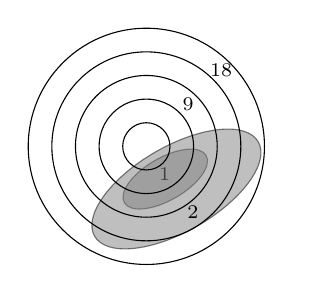
\begin{tikzpicture}[every node/.style={fill=white, font=\sffamily}, align=center,scale=0.6]

    
    \visible<1->{
      \draw[ellipse, rotate=30, fill=gray, opacity=0.5] (0.0, -0.8) ellipse (1.0cm and 0.45cm);
      \node[other, draw=none] at (0.4, -0.6) {$\Rcal_{1}$};
      \draw[ellipse, rotate=30, fill=gray, opacity=0.5] (0.1, -1.1) ellipse (2.0cm and 0.9cm);
      \node[other, draw=none] at (1.0, -1.4) {$\Rcal_{2}$};
    }

    % \visible<2->{
    %   \node[other, draw=none] at (0.20, 0.20) {$\Ccal_{1}$};
    % }

    \visible<2->{
      \draw (0,0) circle (0.5cm);
      \draw (0,0) circle (1.0cm);
      \node[other, draw=none] at (0.55, 0.55) {$\iddots$};
      \node[other, draw=none] at (0.90, 0.90) {$\Ccal_{9}$};
      \draw (0,0) circle (1.5cm);
    }

    \visible<3->{
      \node[other, draw=none] at (1.25, 1.25) {$\iddots$};
      \draw (0,0) circle (2.0cm);
      \node[other, draw=none] at (1.60, 1.60) {$\Ccal_{18}$};
      \draw (0,0) circle (2.5cm);
    }


\end{tikzpicture}

%   \end{minipage}
%
%   {\small
%   \begin{itemize}
%     \item[$\bullet$] <1-> $\Rcal_{k}$: all functions representable by neural networks of total rank at most $k$
%     \item[$\bullet$] <2-> $\Ccal_{p}$: all functions representable by diagonal-circulant networks of depth at most $p$
%    \end{itemize}
%   }
%
% \end{frame}


%%%%%%%%%%%%%%%%%%%%%%%%%%%%%%%%%%%%%%%%%%%%%%%%%%%%%%%%%%%%%%%%%%%%%%%%%%%%%%%
\begin{frame}{Interpretation of the Result}
%%%%%%%%%%%%%%%%%%%%%%%%%%%%%%%%%%%%%%%%%%%%%%%%%%%%%%%%%%%%%%%%%%%%%%%%%%%%%%%

  \begin{minipage}{\textwidth}
    \centering
    \tikzset{%
	 base/.style = {rectangle, draw=black},
	 other/.style = {base, fill=none,  minimum width=1.7cm, minimum height=0.7cm},
       ellipse/.style = {base}
    }
    \begin{tikzpicture}[overlay]

      \foreach \PointA in {-5,-4,-3, -2,-1,0,+1,+2,+3,+4,+5} {
        \foreach \PointB in {-4,-3,-2,-1,0,+1,+2,+3} {
	  \draw [white,fill=white,opacity=0] (\PointA,\PointB) circle (0.02cm);
	 }
      }

      \draw[ellipse, rotate=30, fill=gray, opacity=0.5] (0.0, -0.8) ellipse (1.0cm and 0.45cm);
      \node[other, draw=none] at (0.4, -0.6) {$\Rcal_{1}$};

      \node[fill=none] (msg1) at (-2., -2.) {
        {\footnotesize
        \begin{minipage}{0.35\textwidth}
          \centering
	  Set of all functions representable \\ by a network of total rank $1$
        \end{minipage}}
       };
      \path[->, color=OrangePSL, thick] (msg1.north) edge [bend left] (-0.5, -1);


      \visible<2->{
	\node[fill=none] (msg2) at (-2., 2.) {
	  {\footnotesize
	  \begin{minipage}{0.35\textwidth}
	    \centering
	    Set of all functions representable \\ by a DCNN of depth 1 
	  \end{minipage}}
	 };
	\path[->, color=OrangePSL, thick] (msg2.south) edge [bend right] (-0.5, 0);
	\node[other, draw=none] at (0.05, 0.05) {$\Ccal_{1}$};
        \draw (0,0) circle (0.5cm);
      }

      \visible<3->{
	\node[fill=none] (msg3) at (2.5, 2.5) {
	  {\footnotesize
	  \begin{minipage}{0.40\textwidth}
	    \centering
	    We need a DCNN of depth 9 \\ to represent all functions in $\Rcal_1$
	  \end{minipage}}
	 };
	\path[->, color=OrangePSL, thick] (msg3.south) edge [bend left] (1.3, 0.8);
	\draw (0,0) circle (1.0cm);
	\draw (0,0) circle (1.5cm);
	\node[other, draw=none] at (0.55, 0.55) {$\iddots$};
	\node[other, draw=none] at (0.90, 0.90) {$\Ccal_{9}$};
      }

    \end{tikzpicture}
  \end{minipage}


\end{frame}






%%%%%%%%%%%%%%%%%%%%%%%%%%%%%%%%%%%%%%%%%%%%%%%%%%%%%%%%%%%%%%%%%%%%%%%%%%%%%%%
\begin{frame}{Other Approaches for Structured Neural Networks}
%%%%%%%%%%%%%%%%%%%%%%%%%%%%%%%%%%%%%%%%%%%%%%%%%%%%%%%%%%%%%%%%%%%%%%%%%%%%%%%

  Other approaches for structured neural networks:
  \begin{itemize}
    \item[$\bullet$] Toeplitz Neural networks for robotics ({\color{SkyBlue}{\cite{sindhwani2015structured}}})
    \begin{itemize}
      \item[$\rightarrow$] \small{very small networks with 200 / 300 parameters}
    \end{itemize}
    \item[$\bullet$] Product of Diagonal and Cosine Transform ({\color{SkyBlue}{\cite{moczulski2016acdc}}})
    \begin{itemize}
      \item[$\rightarrow$] \small{only replace the last layer of neural networks}
    \end{itemize}
    \item[$\bullet$] Low Displacement Rank ({\color{SkyBlue}{\cite{thomas2018learning}}})
    \begin{itemize}
      \item[$\rightarrow$] \small{difficult training due to the use of Krylov subspace}
    \end{itemize}
  \end{itemize}

  \vspace{0.5cm}

  % \pause
  % \begin{mdframed}[linecolor=OrangePSL,linewidth=1pt]
  %   \centering
  %   We have trained large scale diagonal circulant neural networks by proving an initialization scheme to avoid vanishing and exploding gradients.	 
  % \end{mdframed}

  \pause
  \begin{mdframed}[linecolor=OrangePSL,linewidth=1pt]
    % \centering
    We have trained diagonal circulant neural networks on \orangebold{large scale tasks}:
    \vspace{-0.2cm}
    \begin{itemize}[leftmargin=7pt]
      \item[$\bullet$] exploiting the properties of circulant matrices
      \item[$\bullet$] devising an initialization scheme to avoid vanishing and exploding gradients
    \end{itemize}
  \end{mdframed}


\end{frame}



%%%%%%%%%%%%%%%%%%%%%%%%%%%%%%%%%%%%%%%%%%%%%%%%%%%%%%%%%%%%%%%%%%%%%%%%%%%%%%%
\begin{frame}{Large-scale Video Classification Task}
%%%%%%%%%%%%%%%%%%%%%%%%%%%%%%%%%%%%%%%%%%%%%%%%%%%%%%%%%%%%%%%%%%%%%%%%%%%%%%%

  \begin{block}{Large Scale Video Classification with the \yt dataset}
    \begin{itemize}
      \item 8 million embedded audio \& video frames
      \item 3200 classes
    \end{itemize}
  \end{block}

  State-of-the-art architecture for video classification ({\color{SkyBlue}{\cite{miech2017learnable}}}).
  \begin{figure}[htb]
    \scalebox{0.65}{\tikzset{%
  >={Latex[width=2mm,length=2mm]},
  % Specifications for style of nodes:
            base/.style = {rectangle, draw=black, text centered, font=\sffamily},
             box/.style = {base, rounded corners, text depth=3cm, minimum height=4cm, minimum width=3cm},
     transparent/.style = {rectangle, draw=black},
       circulant/.style = {base, fill=yellow!30},
       embedding/.style = {base, fill=blue!30, minimum width=2.5cm, minimum height=1cm},
           other/.style = {base, fill=white!30,  minimum width=2cm, minimum height=1cm},
              fc/.style = {base, fill=orange!30, minimum width=1.5cm, minimum height=1cm},
          gating/.style = {base, fill=green!30, minimum width=2cm, text width=2cm, minimum height=1cm},
             moe/.style = {base, fill=purple!30, minimum width=1.5cm, minimum height=1cm},
}

\begin{tikzpicture}[every node/.style={fill=white, font=\sffamily}, align=center]

  % \draw (0.0, +2.)  node [other, draw=none, opacity=0, text opacity=1] {\textbf{Embedding}};
  % \draw (+3.7, +2.)  node [other, draw=none, opacity=0, text opacity=1] {\textbf{Dim Reduction}};
  % \draw (+8.0, +2.)  node [other, draw=none, opacity=0, text opacity=1] {\textbf{Classification}};
  \draw (0.0, +2.)  node [other, draw=none, opacity=0, text opacity=1] {\textbf{Layer 1}};
  \draw (+3.7, +2.)  node [other, draw=none, opacity=0, text opacity=1] {\textbf{Layer 2}};
  \draw (+8.0, +2.)  node [other, draw=none, opacity=0, text opacity=1] {\textbf{Layer 3}};

  \draw (0, +0.8)  node [embedding] {Video};
  \draw (0, -0.8)  node [embedding] {Audio};

  \draw (+2.5, +0.8)  node (fc) [fc] {FC};
  \draw (+2.5, -0.8)  node (fc) [fc] {FC};

  \draw (+4.75, 0)  node (fc) [other] {concat};
  \draw (+7.0, 0)  node (moe) [moe] {MoE};
  \draw (+9.25, 0)  node (gating2) [gating] {Context Gating};
 
  \draw (+1.5, +2) [dashed] -- (+1.5, -1.7);
  \draw (+6, +2) [dashed] -- (+6, -1.7);
  
  % \draw (3.5, -2.6)  node [other, draw=none, opacity=0, text opacity=1] {\textbf{use of Diagonal-Circulant layers}};
  % \draw (0.0, -1.5) -- (2.7, -2.3);
  % \draw (2.5, -1.5) -- (3.3, -2.3);
  % \draw (7.0, -0.8) -- (4.0, -2.3);
  
\end{tikzpicture}
}
  \end{figure}
  $\Rightarrow$ This architecture has 5.7 million parameters.

\end{frame}


%%%%%%%%%%%%%%%%%%%%%%%%%%%%%%%%%%%%%%%%%%%%%%%%%%%%%%%%%%%%%%%%%%%%%%%%%%%%%%%
\begin{frame}{Large-scale Video Classification Task}
%%%%%%%%%%%%%%%%%%%%%%%%%%%%%%%%%%%%%%%%%%%%%%%%%%%%%%%%%%%%%%%%%%%%%%%%%%%%%%%

  \begin{minipage}{\textwidth}
    \centering
    Graph representing the trade-off between accuracy and compression rate.
  \end{minipage}
  \vspace{0.2cm}

  \only<1>{
    \begin{minipage}{\textwidth}
      \centering
      \scalebox{0.8}{\input{graphs/layers_0}}
    \end{minipage}

    \vspace{0.3cm}
    \begin{minipage}{\textwidth}
      \centering
      The original architecture achieves an accuracy GAP of 84\%.
    \end{minipage}
  }

  \only<2>{
    \begin{minipage}{\textwidth}
      \centering
      \scalebox{0.8}{\input{graphs/layers_1}}
    \end{minipage}

    \vspace{0.3cm}
    \begin{minipage}{\textwidth}
      \centering
      We achieve \orangebold{9.2\% compression rate} with \orangebold{no loss} in accuracy.
    \end{minipage}
  }

  \only<3>{
    \begin{minipage}{\textwidth}
      \centering
      \scalebox{0.8}{\begin{tikzpicture}
\begin{axis}[
    width=0.85\textwidth,
    height=0.6\textwidth,
    xlabel={Epochs},
    ylabel={Accuracy GAP},
    xmin=0, xmax=7,
    ymin=0.63, ymax=0.87,
    xtick={0,1,2,3,4,5,6,7},
    ytick={0.63, 0.66, 0.69, 0.72, 0.75, 0.78, 0.81, 0.84, 0.87},
    ymajorgrids=true,
    grid style=dashed,
	]
  \addplot[color=myred!100,  thick, dashed] table [y=gap, x=epoch]{data/layers/dense.dat};
  \addplot[color=NavyBlue!100, thick] table [y=gap, x=epoch]{data/layers/compact_fc.dat};
  \addplot[color=OrangePSL!100, thick] table [y=gap, x=epoch]{data/layers/compact_dbof.dat};
  % \addplot[color=green!100, thick] table [y=gap, x=epoch]{data/layers/compact_moe.dat};

  % \draw [color=myred!100, thick, <-] (axis cs:2.8,0.835) -- +(+10pt,-10pt) node[right] {Original};
  % \draw [color=myred!100, thick, <-] (axis cs:3.0,0.843) -- +(+10pt,+10pt) node[right] {Original};
  % \draw [color=NavyBlue!30,  thick, <-] (axis cs:2.0,0.834) -- +(-10pt,+10pt) node[left]  {9.2\%};
  \draw [color=OrangePSL!100, thick, <-] (axis cs:5.2,0.830) -- +(+10pt,-10pt) node[right] {18.4\%};
  % \draw [color=black!100, thick, <-] (axis cs:5.0,0.800) -- +(+10pt,-10pt) node[right] {72.0\%};



\end{axis}
\end{tikzpicture}
}
    \end{minipage}

    \vspace{0.3cm}
    \begin{minipage}{\textwidth}
      \centering
      We achieve \orangebold{18\% compression rate} with a loss of \orangebold{2 points} in accuracy.
    \end{minipage}
  }

  \only<4>{
    \begin{minipage}{\textwidth}
      \centering
      \scalebox{0.8}{\input{graphs/layers_3}}
    \end{minipage}

    \vspace{0.3cm}
    \begin{minipage}{\textwidth}
      \centering
      We achieve \orangebold{72\% compression rate} with a loss of only \orangebold{4 points} in accuracy.
    \end{minipage}
  }

\end{frame}


